\chapter{Fase geométrica en JCM generalizado}
\label{ch5:fgdoble}


%CAMBIAR ESTO PARA PERSONALIZARLO A MI GUSTO
\pagestyle{fancy}
\fancyhf{}
\fancyhead[LE]{\nouppercase{\rightmark\hfill}}
\fancyhead[RO]{\nouppercase{\leftmark\hfill}}
\fancyfoot[LE,RO]{\hfill\thepage\hfill}
Este capítulo se divide en dos partes. En la primera se estudia la dependencia de la FG con los parámetros del problema, y se analizan situaciones de robustez, intentando ver si las condiciones halladas en el capítulo anterior predicen correctamente dichas características. En la segunda parte, se examina en detalle la robustez para varias condiciones iniciales diferentes, pero siempre en función del detunning, ya que este es el parámetro más accesible experimentalmente.

\section{Dependencias de la FG}

Al igual que en la sección \ref{sec3:jcm disipativo}, se estudia la dependencia de la fase geométrica con los distintos parámetros del problema, siguiendo la definición de la FG en Ec. (\ref{ec2:fg general puro}). Se estudian los efectos en cada caso, y se buscan condiciones de robustez. Nuevamente, se estudian las condiciones iniciales $\frac{1}{\sqrt{2}}(\ket{eg0}+\ket{ge0})$ y $\frac{1}{\sqrt{2}}(\ket{eg1}+\ket{ge1})$, con el objetivo de recuperar comportamientos similares al JCM de 1 átomo para el primer caso, y comparar estos con el otro. 

\subsection{Dependencia con el régimen de acoplamiento}

En la figura \ref{fig5:dependencia acoplamiento} se observa la fase geométrica acumulada para diferentes valores del acoplamiento con el entorno $\gamma=0, 0.01g,0.1g,0.5g,g$, donde cada valor se corresponde con una curva mostrada, en orden ascendente en los colores. Es decir, $\gamma=0$ se corresponde con la curva azul oscuro, y $\gamma=g$ con el color más claro (naranja). El comportamiento para la condición inicial $\frac{1}{\sqrt{2}}(\ket{eg0}+\ket{ge0})$ mostrado en la figura \ref{fig5:dependencia acoplamiento eg0} es idéntico al caso del JCM de 1 átomo, donde aumentar la disipación hace que los escalones se suavicen, y dejen de acumular fase rápidamente por la destrucción de las coherencias. 

\begin{figure}[h]
    \centering
    \begin{subfigure}{0.49\textwidth}
        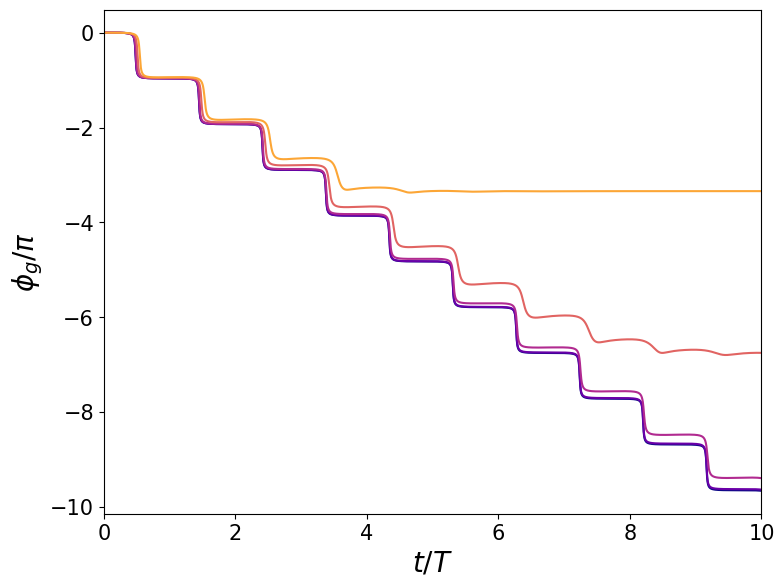
\includegraphics[width=\textwidth]{figuras/ch5/dependencia/eg0+/acoplamiento d=0.1g.png}
        \caption{}
        \label{fig5:dependencia acoplamiento eg0}
    \end{subfigure}
    \hfill
    \begin{subfigure}{0.49\textwidth}
        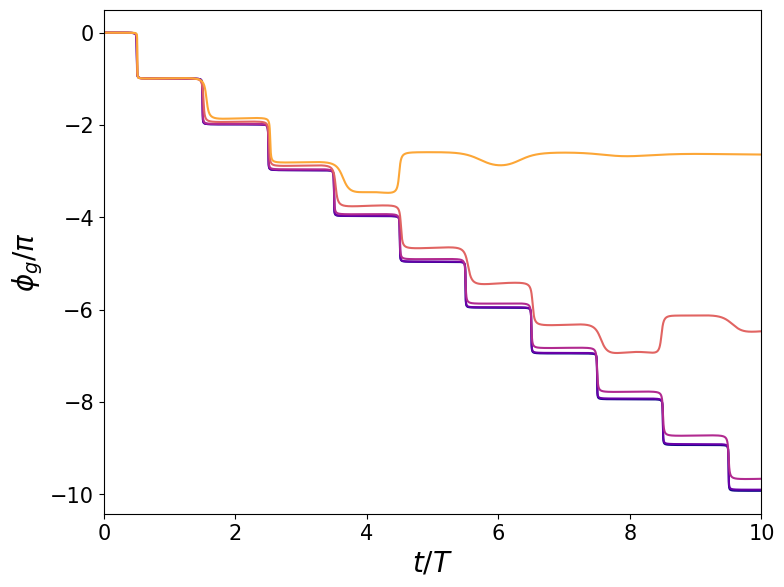
\includegraphics[width=\textwidth]{figuras/ch5/dependencia/eg1+/acoplamiento d=0.1g.png}
        \caption{}
        \label{fig5:dependencia acoplamiento eg1}
    \end{subfigure}
    \caption{Dependencia de la FG acumulada con el acoplamiento con el entorno para condiciones iniciales (a) $\frac{1}{\sqrt{2}}(\ket{eg0}+\ket{ge0})$ y (b) $\frac{1}{\sqrt{2}}(\ket{eg1}+\ket{ge1})$.}
    \label{fig5:dependencia acoplamiento}
\end{figure}
En el caso de la condición inicial correspondiente al subespacio de $N=2$, se observa un nuevo comportamiento: un \textit{rebote}. Al aumentar lo suficiente el acoplamiento con el entorno, la acumulación de fase geométrica hace un salto en la dirección contraria a la que lleva normalmente, y luego oscila cerca a su valor asintótico. Como se vio anteriormente, los saltos que hacen aparecer los escalones, se podían interpretar en el caso de 1 átomo utilizando la esfera de Bloch. Estos saltos ocurren cuando la trayectoria llega al otro lado de la esfera de Bloch. Al llegar al lado opuesto (digamos $\phi=\pi$), justo al superar este punto, el camino más corto para cerrar el ciclo, según la regla de la geodésica, es recorrer la esfera por el otro lado, dando así un salto de $\pi$ en el caso resonante. Esta interpretación en el caso de un espacio de Hilbert más extenso no es tan directa, pero se puede pensar en analogía en una esfera de mayor dimensión, en donde el rebote sería una situación similar a la descrita anteriormente. Más allá de esto, el comportamiento es el esperado, e incluso se ve que ambos casos acumulan una fase geométrica muy similar en términos de su valor absoluto. No parece haber diferencias significativas en la influencia que tiene el entorno sobre estos dos estados.

\subsection{Dependencia con el detunning}
%delta list=(0.00001*g,0.1*g,0.500001*g,1.00001*g,1.500001*g,2.5*g,5*g)

Para estudiar el efecto del detunning sobre la fase geométrica, se dejan fijos los otros parámetros del problema y se varía la diferencia entre las frecuencias de los átomos y la cavidad. Como el régimen de acoplamiento fuerte es el que nos interesa, se elije un acoplamiento con el entorno $\gamma=0.1g$ y $p=0.005g$, y en un principio los demás parámetros en cero $\chi=k-J=0$. En la figura \ref{fig5:dependencia detunning} se muestran la fase acumulada para diferentes valores del detunning $\Delta$ para las dos condiciones iniciales elegidas. En \ref{fig5:dependencia detunning eg0} se observa el mismo comportamiento que en el caso de 1 átomo, el detunning hace que los escalones sean más suaves y el salto menor, haciendo que en conjunto el sistema acumule menos fase geométrica. Si asociamos la fase geométrica al camino que recorre el estado en el espacio de estados, es evidente que a mayor detunning, la fase acumulada será menor, ya que como se mencionó en reiteradas ocasiones, al aumentar el detunning las oscilaciones entre los estados son más pequeñas, y por lo tanto la probabilidad está concentrada en la condición inicial. Consecuentemente, en el espacio de rayos, la curva se mantiene cerca del origen y, por lo tanto, la fase acumulada es menor. En el caso de la condición inicial en el subespacio de $N=2$, si el detunning es bajo, entonces el efecto es similar al anterior y la fase acumulada tiene una forma y un valor similar. Pero aproximadamente en el rango de $1g \leq \Delta \leq 5g$, hay una gran diferencia. La fase acumulada es más errática y presenta saltos y \textit{rebotes}. Al seguir aumentando el detunning, estos parecen disminuir y converger al comportamiento esperado para un detunning grande: que la fase acumulada sea poca.
\begin{figure}[h]
    \centering
    \begin{subfigure}{0.49\textwidth}
        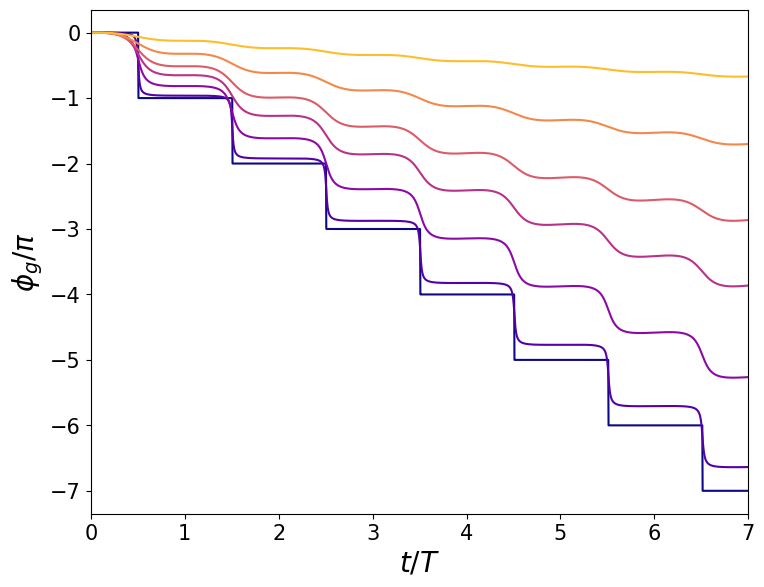
\includegraphics[width=\textwidth]{figuras/ch5/dependencia/eg0+/detunning todo 0.png}
        \caption{}
        \label{fig5:dependencia detunning eg0}
    \end{subfigure}
    \hfill
    \begin{subfigure}{0.49\textwidth}
        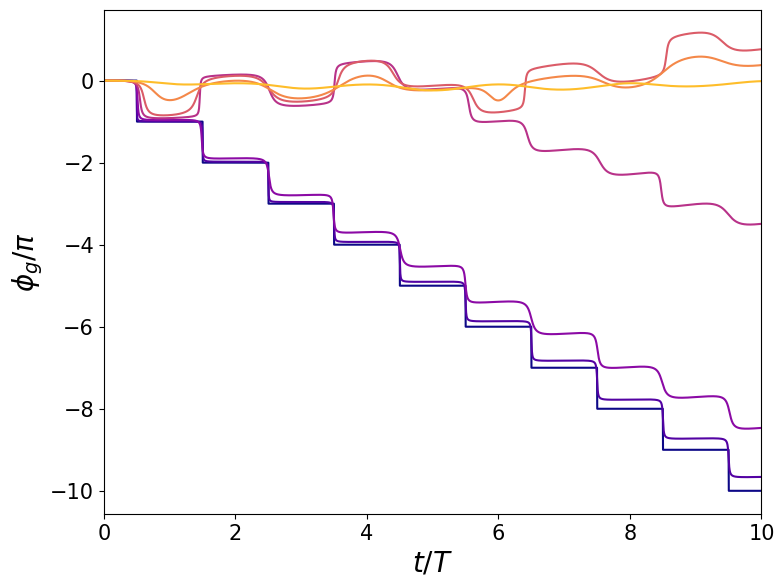
\includegraphics[width=\textwidth]{figuras/ch5/dependencia/eg1+/detunning todo 0.png}
        \caption{}
        \label{fig5:dependencia detunning eg1}
    \end{subfigure}
    \caption{Dependencia de la FG acumulada con el detunning para condiciones iniciales (a) $\frac{1}{\sqrt{2}}(\ket{eg0}+\ket{ge0})$ y (b) $\frac{1}{\sqrt{2}}(\ket{eg1}+\ket{ge1})$.}
    \label{fig5:dependencia detunning}
\end{figure}
Una explicación para el comportamiento en el rango medio de detunning es que las poblaciones comienzan a presentar batidos. Las probabilidades de los estados $\ket{ee0}$ y $\ket{gg2}$ comienzan a aumentar y son comparables a la probabilidad del estado inicial. Esto hace que en el espacio de estados, las curvas sean complicadas y tengan trayectorias largas, haciendo que en algunos casos el salto sea positivo, y en otros, negativo. Para valores de detunning bajos, el sistema principalmente se centra en el estado $\frac{1}{\sqrt{2}}(\ket{eg1}+\ket{ge1})$, y para detunnings altos también. Es en este rango intermedio, que las amplitudes de los 3 estados sin similares y oscilan de manera errática, presentando batidos, y por eso la fase geométrica acumulada no sigue un comportamiento continuo a lo largo de su dependencia con el parámetro. 
No se encontró una manera clara de representar ésto en el espacio de parámetros para poder entender intuitivamente el comportamiento, ya que la esfera de Bloch no es una herramienta que se pueda utilizar en esta situación. 
Para seguir el estudio, se presenta la diferencia entre la fase geométrica unitaria y la disipativa en función del detunning. Para ello se realizan simulaciones para diferentes valores de $\Delta$ y se compara el valor de la fase geométrica luego de un tiempo fijo $t=3T$ para dos casos, el primero presentando pérdidas y el segundo sin pérdidas. Luego se realiza la resta de ambas cantidades y se obtiene el gráfico \ref{fig5:robustez detunning eg0}.

\begin{figure}[h]
    \centering
    \begin{subfigure}{0.49\textwidth}
        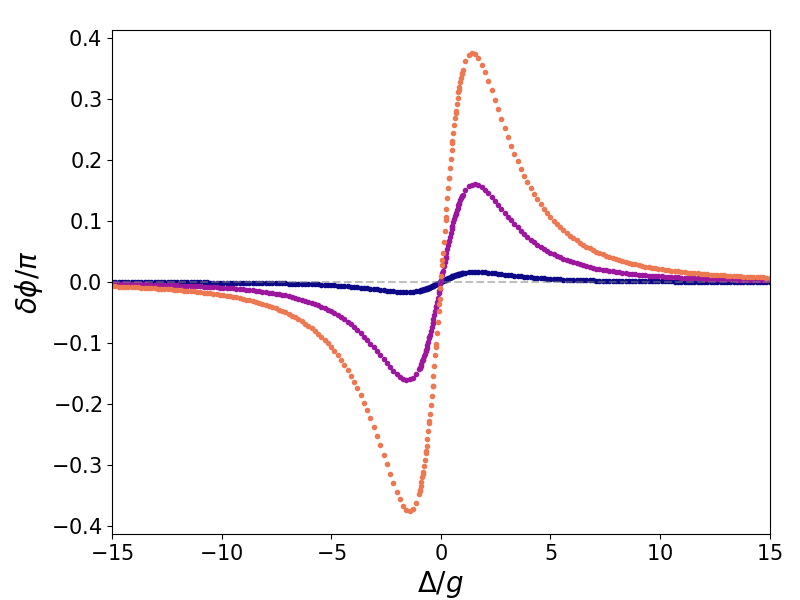
\includegraphics[width=\textwidth]{figuras/ch5/robustez/delta/eg0+ge0 k=0.0g x=0.0g J=0.0g.png}
        \caption{}
        \label{fig5:robustez detunning 1 eg0}
    \end{subfigure}
    \hfill
    \begin{subfigure}{0.49\textwidth}
        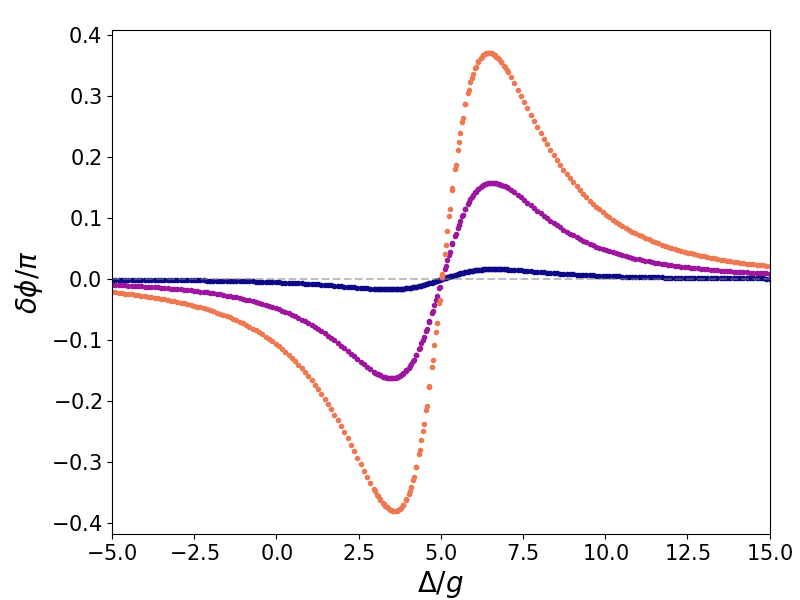
\includegraphics[width=\textwidth]{figuras/ch5/robustez/delta/eg0+ge0 k=0.0g x=5.0g J=0.0g.png}
        \caption{}
        \label{fig5:robustez detunning 2 eg0}
    \end{subfigure}
    \vfill

    \caption{Robustez en funcion de $\Delta$ para la condición inicial $\frac{1}{\sqrt{2}}(\ket{eg0}+\ket{ge0})$ para (a) $\chi=0$ y (b) $\chi=5g$.}
    \label{fig5:robustez detunning eg0}
\end{figure}

En este gráfico se muestran tres curvas diferentes correspondientes a tres valores diferentes del acoplamiento con el entorno, respectivamente caracterizados por $\gamma=0.01g,0.1g$ y $0.25g$, y la condición inicial $\frac{1}{\sqrt{2}}(\ket{eg0}+\ket{ge0})$. En primer lugar, se ve que las curvas pasan por el origen, lo que nos dice que la diferencia entre la fase geométrica en ambos casos es 0, que es lo que llamamos condición de robustez, ya que el entorno no tiene efecto sobre la fase geométrica y esta se mantiene robusta ante los efectos del entorno. En el panel \ref{fig5:robustez detunning 1 eg0}, correspondiente a $\chi=k-J=0$, la condición de robustez se da para $\Delta=0$, como era de esperarse, ya que es la misma que para el caso de 1 átomo. De la misma manera, al observar el caso de $\chi=5g$ en la figura \ref{fig5:robustez detunning 2 eg0}, esta condición se da para $\Delta=\chi=5g$, que también es lo que se espera.
\begin{figure}[h]
    \centering
    \begin{subfigure}{0.49\textwidth}
        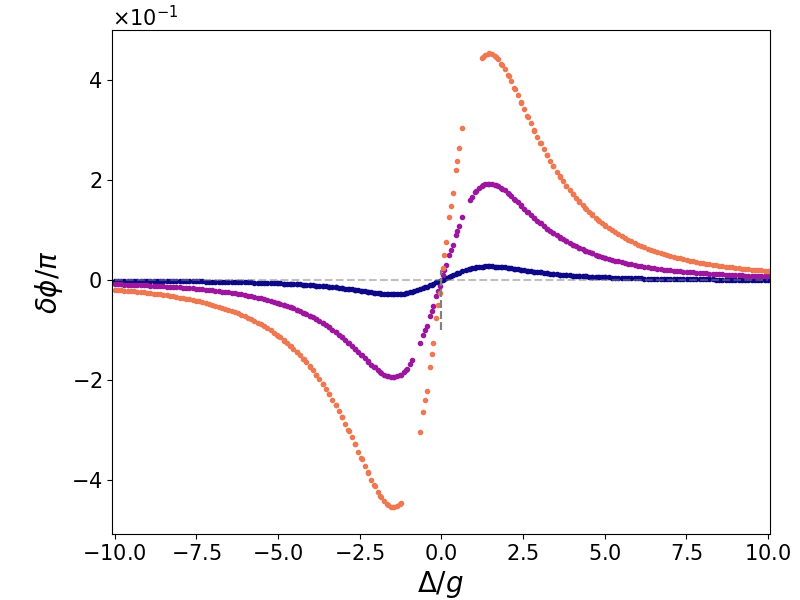
\includegraphics[width=\textwidth]{figuras/ch5/robustez/delta/eg1+ge1 k=0.0g x=0.0g J=0.0g.png}
        \caption{}
        \label{fig5:robustez detunning 1 eg1}
    \end{subfigure}
    \hfill
    \begin{subfigure}{0.49\textwidth}
        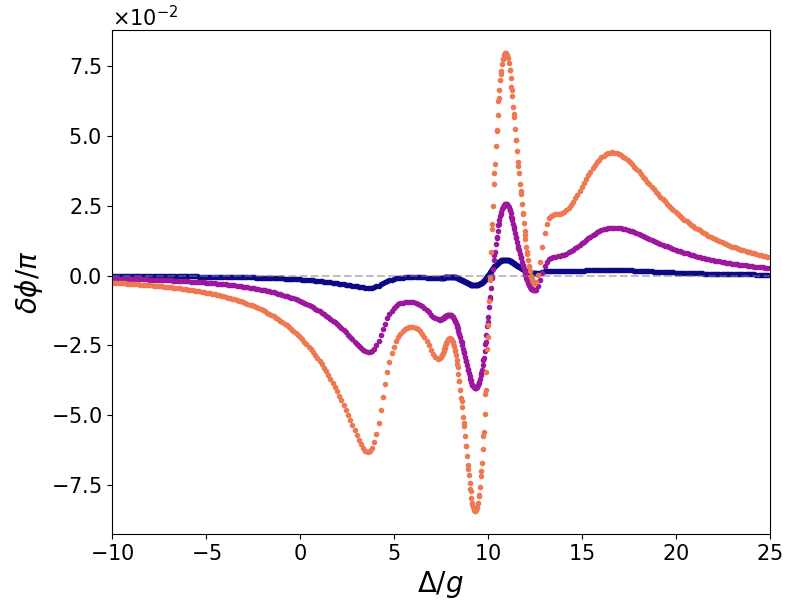
\includegraphics[width=\textwidth]{figuras/ch5/robustez/delta/eg1+ge1 k=0.0g x=5.0g J=0.0g.png}
        \caption{}
        \label{fig5:robustez detunning 2 eg1}
    \end{subfigure}
    \caption{Robustez en función de $\Delta$ para la condición inicial $\frac{1}{\sqrt{2}}(\ket{eg1}+\ket{ge1})$ para (a) $\chi=0$ y (b) $\chi=5g$}
    \label{fig5:robustez detunning eg1}
\end{figure}
La figura \ref{fig5:robustez detunning eg1} muestra la robustez para el estado inicial $\frac{1}{\sqrt{2}}(\ket{eg1}+\ket{ge1})$, sin interacción entre átomos, y para (\ref{sub@fig5:robustez detunning 1 eg1}) $\chi=0$ y (\ref{sub@fig5:robustez detunning 2 eg1}) $\chi=5g$. Con $\chi=0$, no cambia nada con respecto al caso de $N=1$. Pero cuando $\chi=5g$ se observan comportamientos nuevos: (i) hay máximos y mínimos nuevos que dependen suavemente de los parámetros y (ii) hay más de un valor para el cual la diferencia es 0 que además (iii) las condiciones de robustez no predicen correctamente. Para $\Delta=10g$ hay un punto de robustez, correspondiente a la condición dada por Ec. (\ref{ec4:condicion 3}) $\Delta=2\chi$, donde las tres curvas presentan una raíz. Pero también para $\Delta \approx 12.5g$ se observan otras raíces. El mínimo en esta zona depende del acoplamiento con el entorno, y sorprendentemente, para valores de $\gamma=0.1g$ y $\gamma=0.25g$, hay dos raíces, mientras que para $\gamma=0.01g$ no. Si bien las condiciones propuestas logran predecir el caso de robustez, es evidente que el efecto del entorno no se está teniendo en cuenta y puede llevar a comportamientos inesperados. Las dos evidencias más concretas de esto es que, por un lado, la condición de robustez predice correctamente pero con un muy pequeño error ocasionado por el corrimiento de frecuencias por el entorno, y por el otro lado, como se observó en este caso, hay algunos ceros nuevos de la función que aparecen al cambiar el acoplamiento con el entorno. Estos ceros no son condiciones de robustez, ya que suceden \textit{accidentalmente}, en el sentido que justo en el tiempo que se está observando la diferencia, la FG unitaria y disipativa coinciden, pero no en todo tiempo.


\subsection{Dependencia con el medio Kerr}
%chi list=(0.0001*g,0.1*g,0.5*g,g,2*g,5*g)

En el caso de 1 átomo se observó que el efecto del medio sobre la fase es análoga al detunning, y en el caso de dos átomos, se observa en la figura \ref{fig5:dependencia kerr eg0} la condición inicial $\frac{1}{\sqrt{2}}(\ket{eg0}+\ket{ge0})$ que esto sigue siendo cierto para el subespacio de $N=1$. Pero en el caso de la figura \ref{fig5:dependencia kerr eg1} se muestra que el efecto sobre la condición inicial $\frac{1}{\sqrt{2}}(\ket{eg1}+\ket{ge1})$, en comparación con la figura \ref{fig5:dependencia detunning eg1}, muestra diferencias en el régimen intermedio que se había definido aproximadamente para valores entre $1g \leq \chi \leq 5g$. Si bien la forma no es igual, es notable que el rango que se definió como \textit{intermedio} es el mismo. Entonces, si bien para $N=2$ el medio Kerr no es simplemente un corrimiento en el detunning, el comportamiento es similar. 

\begin{figure}[h]
    \centering
    \begin{subfigure}{0.49\textwidth}
        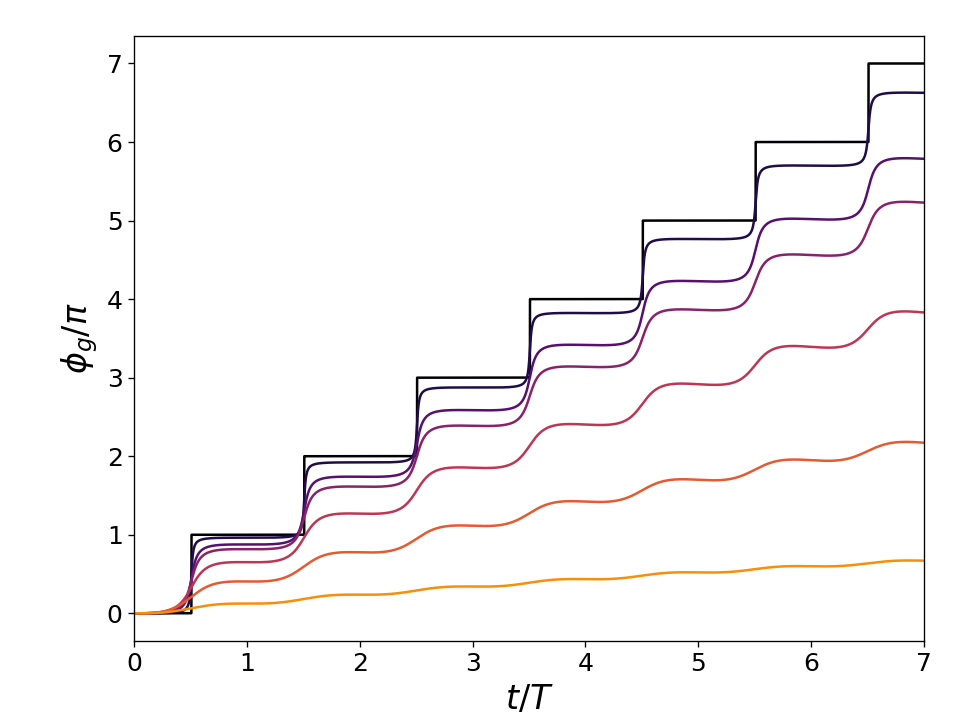
\includegraphics[width=\textwidth]{figuras/ch5/dependencia/eg0+/kerr todo 0.png}
        \caption{}
        \label{fig5:dependencia kerr eg0}
    \end{subfigure}
    \hfill
    \begin{subfigure}{0.49\textwidth}
        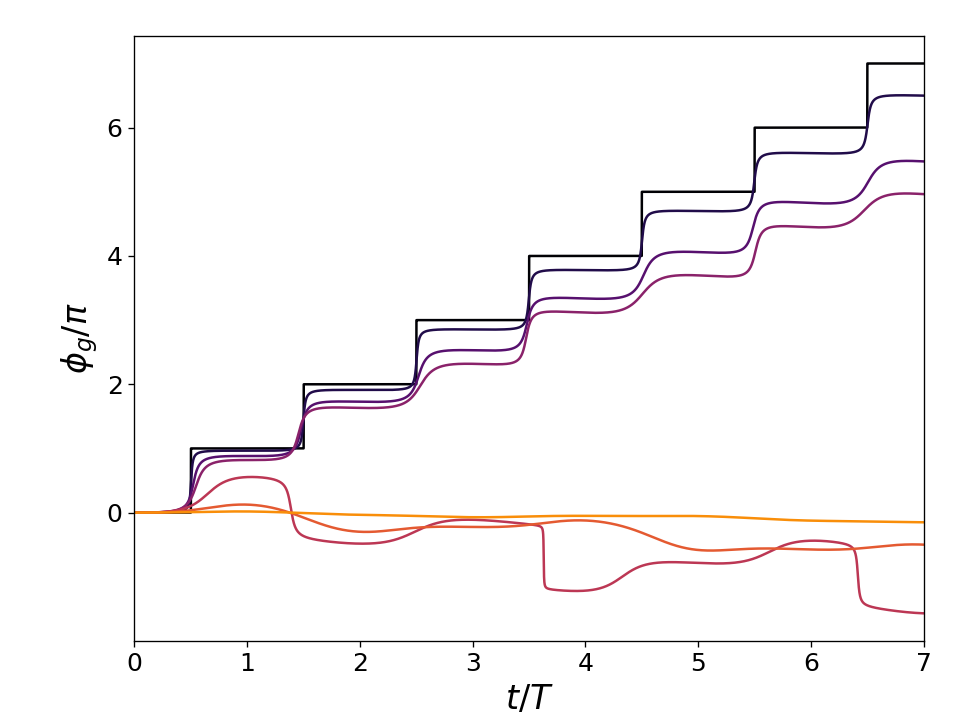
\includegraphics[width=\textwidth]{figuras/ch5/dependencia/eg1+/kerr todo 0.png}
        \caption{}
        \label{fig5:dependencia kerr eg1}
    \end{subfigure}
    \caption{Dependencia de la FG acumulada con el medio Kerr para condiciones iniciales (a) $\frac{1}{\sqrt{2}}(\ket{eg0}+\ket{ge0})$ y (b) $\frac{1}{\sqrt{2}}(\ket{eg1}+\ket{ge1})$.}
    \label{fig5:dependencia kerr}
\end{figure}

La pregunta que surge de todas formas es, qué sucede si se realiza un corrimiento en el detunning. En el caso de 1 átomo se había observado cómo la condición de robustez se cumplía cuando $\Delta=\chi(2n-1)$, y la dependencia de la fase geométrica parecía no cambiar, solo presentaba un corrimiento. 

En la figura \ref{fig5:dependencia kerr 2 eg0} se observa cómo en el primer caso, aumentar el detunning hace que las primeras cuatro curvas, que representan valores de $\chi=0,\;g/10,\;g/6\; y\;g/4$ (en negro y violeta oscuro respectivamente), acumulan fase negativa y los saltos son suaves. Ahora, la curva de $\chi=\Delta=0.5g$ (línea violeta claro) es igual a la de $\chi=\Delta=0$ de la figura \ref{fig5:dependencia kerr eg0}, y a partir de esta, al seguir aumentando el detunning el comportamiento es el mismo que antes. Pero para el caso de $N=2$, ya no es así. Primero, para $\chi=0$ y $\chi=0.1g$ las curvas presentan saltos más abruptos, y hay un rebote. Por otro lado, el caso robusto ya no se observa para $\chi=0.5g$. Ahora, la curva violeta oscura, que representa un valor de $\chi=\frac{\Delta}{3}=g/6$, si bien no es el caso robusto, es muy similar. Se probó por inspección y el valor encontrado para la robustez se dio para $\chi=0.37\Delta$. Esto coincide aproximadamente con la condición de la Ec. (\ref{ec4:condicion 3}). Si se sigue aumentando el valor de $\chi$, en el rango intermedio las oscilaciones de la fase parecen tener más de una componente en frecuencia. Esto se observa claramente en la curva roja, donde se ve que hay dos saltos diferentes. 

\begin{figure}[h]
    \centering
    \begin{subfigure}{0.49\textwidth}
        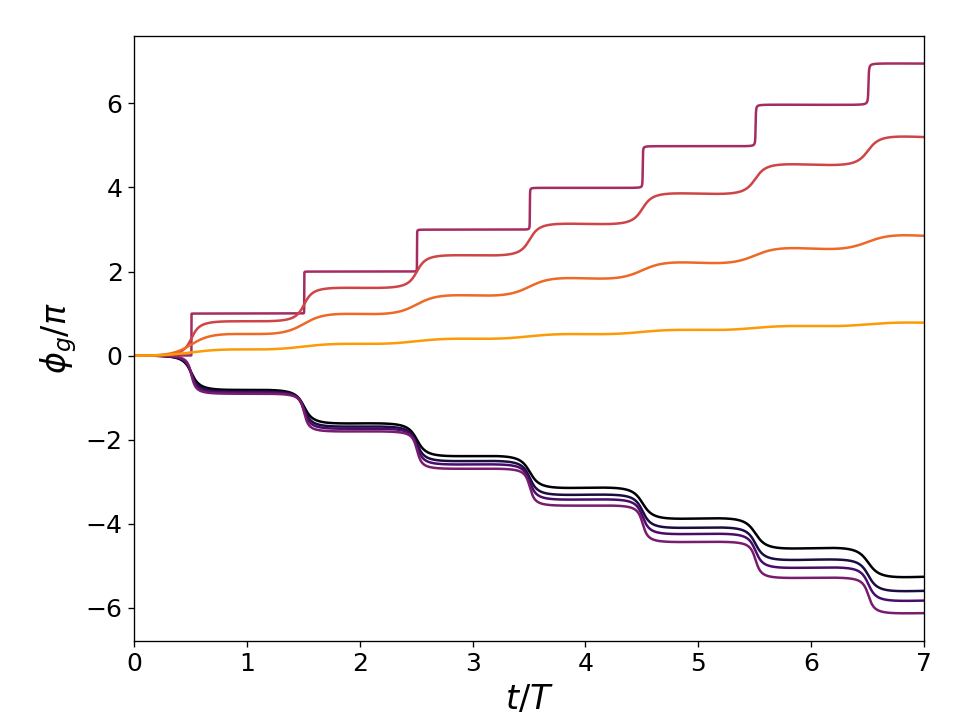
\includegraphics[width=\textwidth]{figuras/ch5/dependencia/eg0+/ker d=0.5g.png}
        \caption{}
        \label{fig5:dependencia kerr 2 eg0}
    \end{subfigure}
    \hfill
    \begin{subfigure}{0.49\textwidth}
        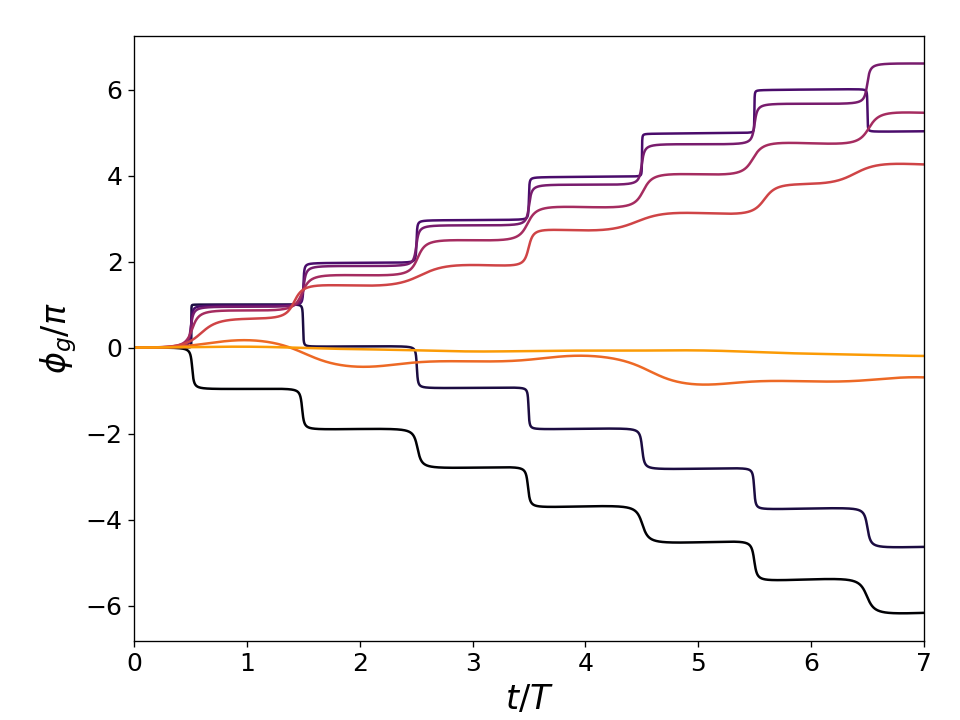
\includegraphics[width=\textwidth]{figuras/ch5/dependencia/eg1+/kerr d=0.5g.png}
        \caption{}
        \label{fig5:dependencia kerr 2 eg1}
    \end{subfigure}
    \caption{Dependencia de la FG acumulada con el medio Kerr con $\Delta=0.5g$ para condiciones iniciales (a) $\frac{1}{\sqrt{2}}(\ket{eg0}+\ket{ge0})$ y (b) $\frac{1}{\sqrt{2}}(\ket{eg1}+\ket{ge1})$.}
    \label{fig5:dependencia kerr 2}
\end{figure}

Finalmente, se realiza un gráfico de diferencias entre la FG unitaria y la disipativa en función del parámetro $\chi$. En la figura \ref{fig5:robustez kerr eg0} se muestra la diferencia $\delta\phi=\phi_d-\phi_u$ para la condición inicial $\frac{1}{\sqrt{2}}(\ket{eg0}+\ket{ge0})$. Se ve cómo la condición de robustez en este caso es igual que para el modelo de 1 átomo, donde la condición se da para $\Delta=\chi$. 

\begin{figure}[h]
    \centering
    \begin{subfigure}{0.49\textwidth}
        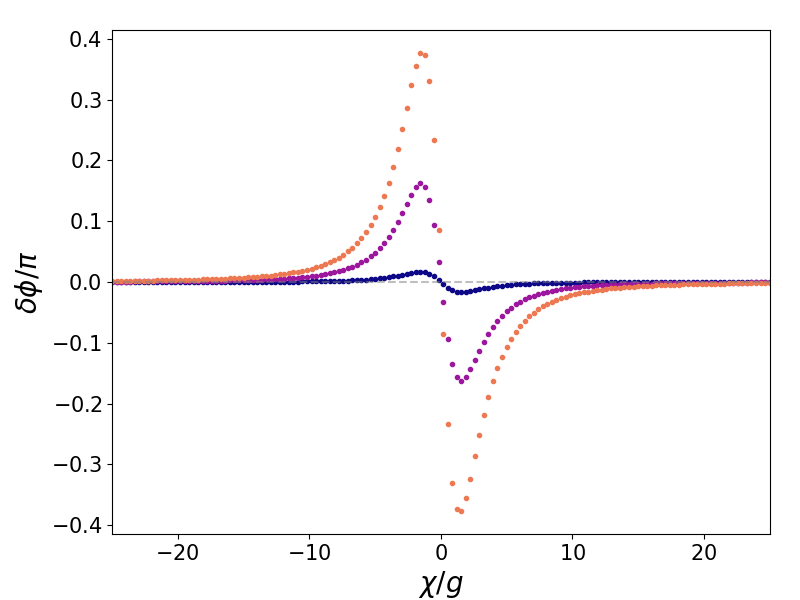
\includegraphics[width=\textwidth]{figuras/ch5/robustez/chi/eg0+ge0 d=0.0g k=0.0g J=0.0g.png}
        \caption{}
        \label{fig5:robustez kerr 1 eg0}
    \end{subfigure}
    \hfill
    \begin{subfigure}{0.49\textwidth}
        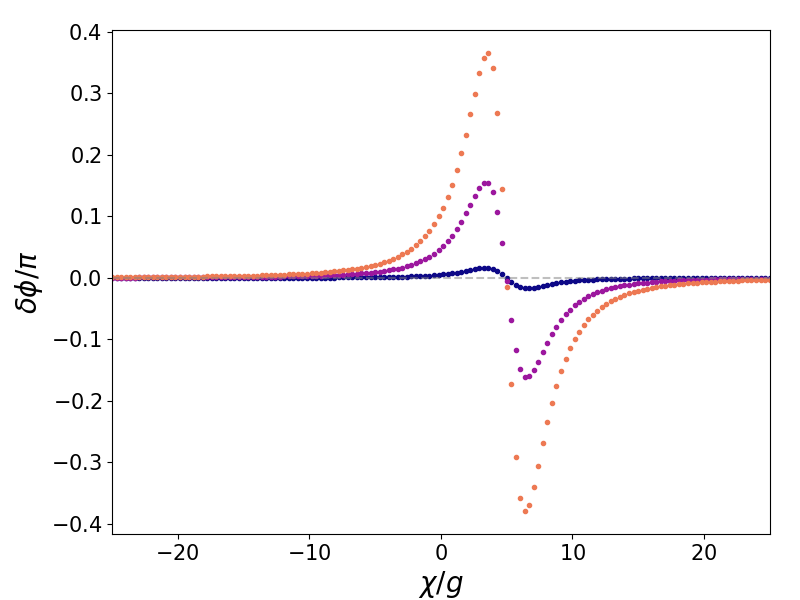
\includegraphics[width=\textwidth]{figuras/ch5/robustez/chi/eg0+ge0 d=5.0g k=0.0g J=0.0g.png}
        \caption{}
        \label{fig5:robustez kerr 2 eg0}
    \end{subfigure}
    \caption{Robustez en función de $\chi$ para la condición inicial $\frac{1}{\sqrt{2}}(\ket{eg0}+\ket{ge0})$ con (a) $\Delta=0$ y (b) $\Delta=5g$}
    \label{fig5:robustez kerr eg0}
\end{figure}

Para la condición inicial $\frac{1}{\sqrt{2}}(\ket{eg1}+\ket{ge1})$ se muestra la figura \ref{fig5:robustez kerr eg1}. Primero, en el panel (\ref{sub@fig5:robustez kerr 1 eg1}) se muestra el caso de $\Delta=0$. La única raíz se da para $\chi=\Delta=0$.

\begin{figure}[h]
    \centering
    \begin{subfigure}{0.49\textwidth}
        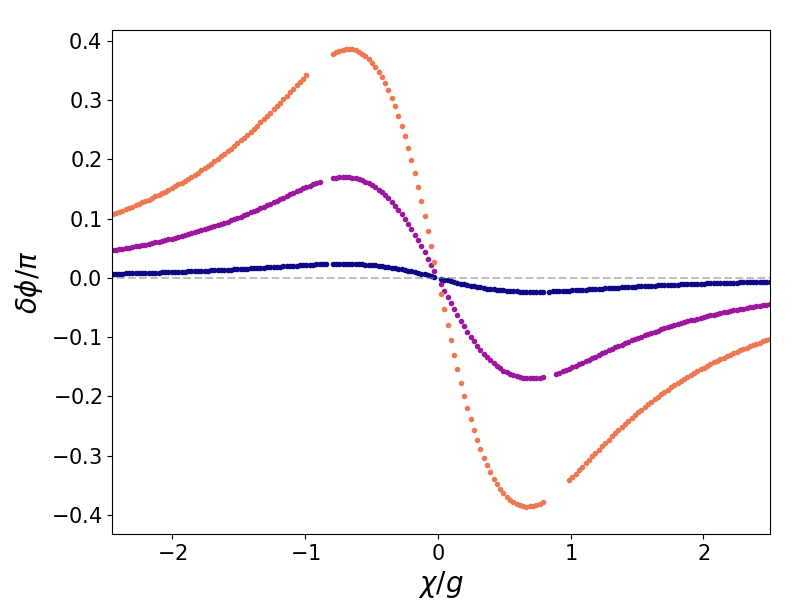
\includegraphics[width=\textwidth]{figuras/ch5/robustez/chi/eg1+ge1 chi zoom.png}
        \caption{}
        \label{fig5:robustez kerr 1 eg1}
    \end{subfigure}
    \hfill
    \begin{subfigure}{0.49\textwidth}
        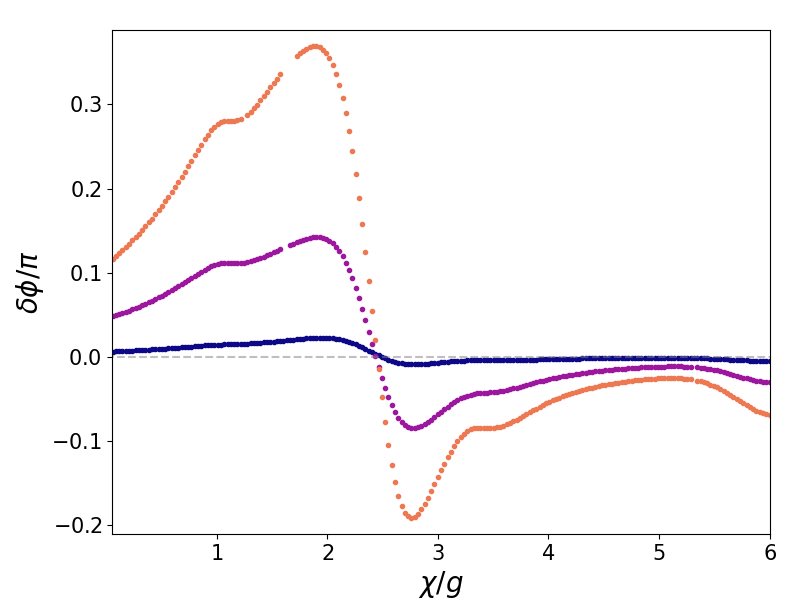
\includegraphics[width=\textwidth]{figuras/ch5/robustez/chi/eg1+ge1 chi d=5.0g.png}
        \caption{}
        \label{fig5:robustez kerr 2 eg1}
    \end{subfigure}
    \caption{Robustez en función de $\chi$ para la condición inicial $\frac{1}{\sqrt{2}}(\ket{eg1}+\ket{ge1})$ con $k-J=0$ y (a) $\Delta=0$; (b) $\Delta=5g$}
    \label{fig5:robustez kerr eg1}
\end{figure}

Hay que aclarar parte de las curvas donde no tienen puntos. En estos casos lo que sucede es que el entorno introduce un corrimiento en las frecuencias. Consecuentemente, hay un pequeño cambio entre la fase unitaria y la no unitaria. En principio, esto no es un problema, ya que lo único que hace es retrasar un poco el escalón. Pero en combinación con la dinámica complicada del sistema, lo que ocurre en casos muy puntuales, es que la fase unitaria y la disipativa hacen un escalón en direcciones contrarias y la diferencia entre ambas presenta un salto abrupto. En la figura \ref{fig5:robustez kerr 1 eg1} cerca de los valores $\chi/g=\pm 1$ se observan la falta de puntos, estos están más arriba por el salto que se mencionó. Es también interesante, que no es solo para un caso aislado, sino que es en un rango de valores donde se observa este comportamiento. 

En la figura \ref{fig5:robustez kerr 2 eg1} se muestra el caso en donde se aumentó el detunning hasta $\Delta=5g$. Se observan máximos y mínimos locales, y la condición de robustez parece estar cercana a $\chi\simeq 2.45g$ y varía suavemente con cada valor de $\gamma$. Esto es muy interesante, ya que el efecto que tiene el entorno también se refleja en esta condición. Nuevamente, esta condición en el subespacio de $N=2$ se da cuando $\Delta=2\chi$ (Ec. (\ref{ec4:condicion 3})), y en la figura \ref{fig4:concu x 1 d2} se observa que para $\chi\simeq2.5g$ también la concurrencia presenta una franja robusta. Algo interesante es que la franja observada en la concurrencia, no es de una gran amplitud, aun así, la fase geométrica presenta una raíz para este caso. Si bien esto es un indicio de que la fase geométrica y la concurrencia están relacionadas, es evidente que hay un mecanismo más fundamental que genera este comportamiento y que será motivo de estudio en el futuro.

\subsection{Dependencia con la interacción entre átomos}
Finalmente, se considera la dependencia en la interacción entre los átomos $k-J$. En la figura \ref{fig5:dependencia interaccion} nuevamente se muestran las dos condiciones iniciales (a) $\frac{1}{\sqrt{2}}(\ket{eg0}+\ket{ge0})$ y (b) $\frac{1}{\sqrt{2}}(\ket{eg1}+\ket{ge1})$. En ambos casos el comportamiento es el mismo. Al aumentar la interacción, la FG acumulada es menor y los saltos son más suaves. A diferencia con el detunning y con el medio, no se reconoce un rango intermedio para el cual el comportamiento sea diferente. 

\begin{figure}[h]
    \centering
    \begin{subfigure}{0.49\textwidth}
        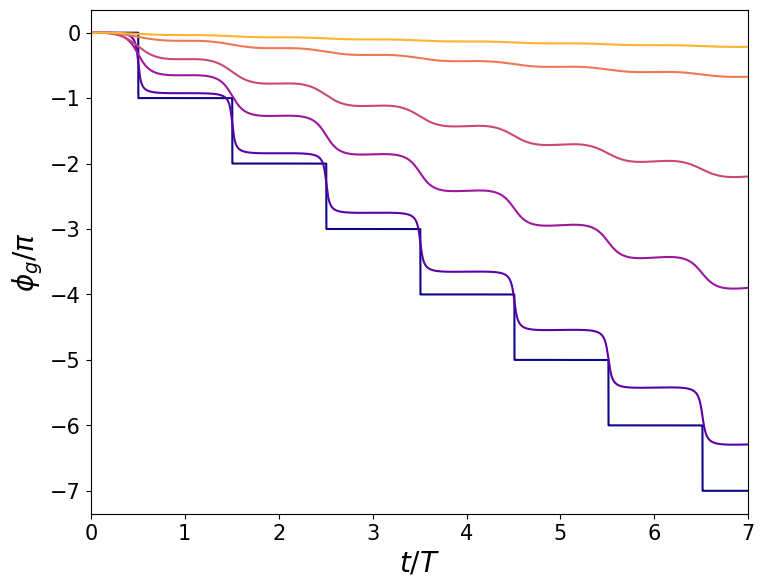
\includegraphics[width=\textwidth]{figuras/ch5/dependencia/eg0+/interaccion todo 0.png}
        \caption{}
        \label{fig5:dependencia interaccion eg0}
    \end{subfigure}
    \hfill
    \begin{subfigure}{0.49\textwidth}
        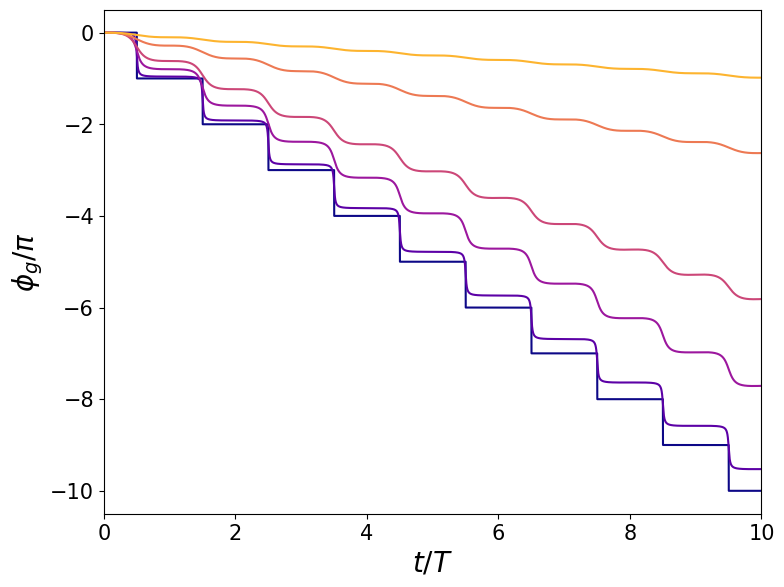
\includegraphics[width=\textwidth]{figuras/ch5/dependencia/eg1+/interaccion todo 0.png}
        \caption{}
        \label{fig5:dependencia interaccion eg1}
    \end{subfigure}
    \caption{Dependencia de la FG acumulada con la interacción entre los átomos $k-J$ para condiciones iniciales (a) $\frac{1}{\sqrt{2}}(\ket{eg0}+\ket{ge0})$ y (b) $\frac{1}{\sqrt{2}}(\ket{eg1}+\ket{ge1})$.}
    \label{fig5:dependencia interaccion}
\end{figure}
En la figura \ref{fig5:robustez interaccion eg0} se muestra la diferencia entre la FG unitaria y disipativa para la condición inicial $\frac{1}{\sqrt{2}}(\ket{eg0}+\ket{ge0})$. El comportamiento es el esperado: la condición de robustez se da cuando $k-J=\frac{\chi-\Delta}{2}$. Nuevamente, los máximos dependen suavemente de los parámetros, y en particular dependen del entorno $\gamma$. 
\begin{figure}[h]
    \centering
    \begin{subfigure}{0.49\textwidth}
        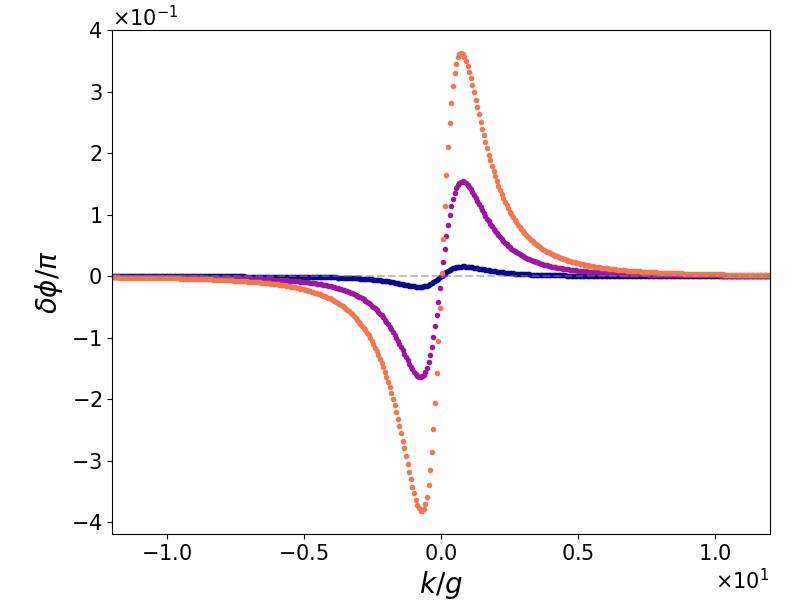
\includegraphics[width=\textwidth]{figuras/ch5/robustez/k/eg0+ge0 d=2.5g x=2.5g J=0.0g.png}
        \caption{}
        \label{fig5:robustez interaccion 1 eg0}
    \end{subfigure}
    \hfill
    \begin{subfigure}{0.49\textwidth}
        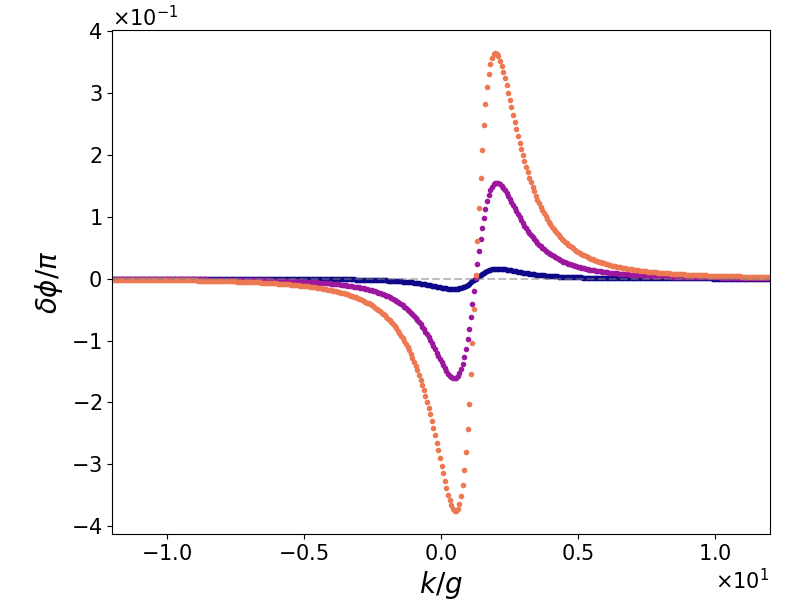
\includegraphics[width=\textwidth]{figuras/ch5/robustez/k/eg0+ge0 d=0.0g x=2.5g J=0.0g.png}
        \caption{}
        \label{fig5:robustez interaccion 2 eg0}
    \end{subfigure}
    \caption{Robustez en función de $\chi$ para la condición inicial $\frac{1}{\sqrt{2}}(\ket{eg0}+\ket{ge0})$ con $\Delta=0$ y (a) $\chi=0$; (b) $\chi=2.5g$}
    \label{fig5:robustez interaccion eg0}
\end{figure}

Para la condición inicial $\frac{1}{\sqrt{2}}(\ket{eg1}+\ket{ge1})$ se muestra la figura \ref{fig5:robustez interaccion eg1}. Cuando $\Delta=\chi=0$ (\ref{sub@fig5:robustez interaccion 1 eg0}), la dependencia parece ser la misma que en el caso de $\frac{1}{\sqrt{2}}(\ket{eg0}+\ket{ge0})$, pero en este caso la fase acumulada es menor por casi 1 orden de magnitud. 
\begin{figure}[h]
    \centering
    \begin{subfigure}{0.49\textwidth}
        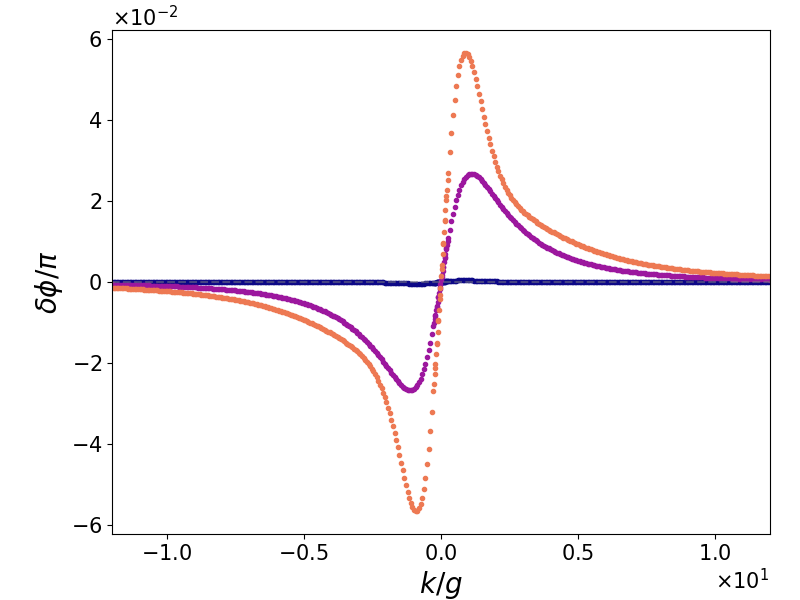
\includegraphics[width=\textwidth]{figuras/ch5/robustez/k/eg1+ge1 d=0.0g x=0.0g J=0.0g.png}
        \caption{}
        \label{fig5:robustez interaccion 1 eg1}
    \end{subfigure}
    \hfill
    \begin{subfigure}{0.49\textwidth}
        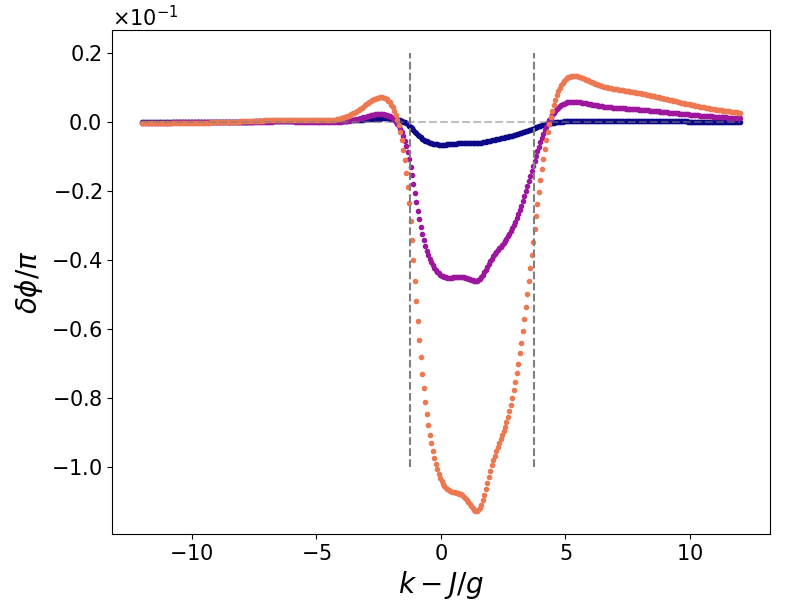
\includegraphics[width=\textwidth]{figuras/ch5/robustez/k/eg1+ge1 d=0.0g x=2.5g J=0.0g.png}
        \caption{}
        \label{fig5:robustez interaccion 2 eg1}
    \end{subfigure}
    \caption{Robustez en función de $\chi$ para la condición inicial $\frac{1}{\sqrt{2}}(\ket{eg1}+\ket{ge1})$ con $\Delta=0$ y (a) $\chi=0$; (b) $\chi=2.5g$}
    \label{fig5:robustez interaccion eg1}
\end{figure}
En la figura \ref{fig5:robustez interaccion 2 eg1} se muestra el caso en que $\Delta=0$ y $\chi=2.5g$. De las tres condiciones de robustez, la condición $\Delta-\chi(2n-2)$ (\ref{ec4:condicion 3}) no puede cumplirse nunca. 

Es interesante que en los casos estudiados anteriormente, en general, era esta la condición que predecía la condición de robustez. Como en este caso no es posible cumplir esta condición, entonces se ve que las otras dos condiciones actúan como condiciones de robustez, que se dan cuando $k-J=-\frac{\chi}{2}$ (Ec. (\ref{ec4:condicion 2})) y $k-J=\frac{3}{2}\chi$ (Ec. (\ref{ec4:condicion 1})). En este caso, en particular son para $k-J=-1.25g$ y $k-J=4.75g$, valores que se marcan con líneas rayadas. Si bien la predicción no es exacta, es bastante buena para aproximar. La discrepancia entre valor predicho y valor observado en las figuras se debe a que no se tuvo en cuenta el efecto del entorno a la hora de conseguir estas condiciones. Otra evidencia de esto es que el cero de cada una de las tres funciones, cuyos valores de $\gamma$ son diferentes, varían suavemente. 

\section{Robustez en función del detunning}

Finalmente, se explora más en detalle las condiciones de robustez dadas por las Ecs. (\ref{ec4:condicion 1})-(\ref{ec4:condicion 3}) en función del detunning. Esto es importante, ya que este es en general el parámetro de control al que se tiene acceso en los experimentos, en general, cambiando la frecuencia de la cavidad. 

Ya se vio que las condiciones de robustez (\ref{ec4:condicion 1})-(\ref{ec4:condicion 3}) predicen correctamente, con cierto error por el efecto del entorno, cuando la diferencia entre la FG unitaria y en sistema abierto es nula. Esto es uno de los resultados más importantes del trabajo, y se quiere estudiar si estas condiciones se cumplen en todos los casos, ya que si bien en los gráficos mostrados por ahora siempre se cumplió, no fueron demasiadas las combinaciones de parámetros estudiados. Lo que se va a hacer en esta sección, es realizar gráficos de robustez como se hicieron anteriormente, pero para un valor fijo del acoplamiento con el entorno $\gamma=0.25g$. También, ya que las condiciones de robustez que se encontraron salieron de pedir degeneración entre las energías de los estados de la base Ec. (\ref{ec4:base}), entonces se quiere ver qué pasa con las otras dos condiciones iniciales del subespacio de $N=2$, que son $\ket{gg2}$ y $\ket{ee0}$.

En la figura \ref{fig5:raices} se muestran los casos de robustez para las condiciones iniciales $\ket{gg2}$ mostradas con el número 1 en celeste, $\frac{1}{\sqrt{2}}(\ket{eg1}+\ket{ge1})$ con un número 2 en gris, y $\ket{ee0}$ con un número 3 en negro. Las tres líneas representan las tres condiciones de robustez (Ecs. (\ref{ec4:condicion 1})-(\ref{ec4:condicion 3}), para diferentes valores de $k-J$. En general, los casos robustos caen sobre las líneas predichas, y en su gran mayoría cada estado inicial respeta consistentemente alguna de las condiciones. Por ejemplo, los estados iniciales $\ket{gg2}$ y $\frac{1}{\sqrt{2}}(\ket{eg1}+\ket{ge1})$ respetan la condición $\Delta=2\chi$, y el estado inicial $\ket{ee0}$ respeta la condición de robustez $\Delta=\chi+2(k-J)$. Esto se cumple en la gran mayoría de los casos, pero como se observa en el caso de $k-J=2.5g$ (panel (c)), el estado inicial $\ket{gg2}$ en un principio respetaba la condición $\Delta=3\chi-2(k-J)$, pero luego este comportamiento cambió. 

Como se mencionó anteriormente, hay pequeñas discrepancias gracias al efecto del entorno. Para cuantificar estas diferencias, se realizó un ajuste lineal, y se obtiene que en presencia del entorno las condiciones se modifican un poco.
\begin{figure}[h]
    \centering
    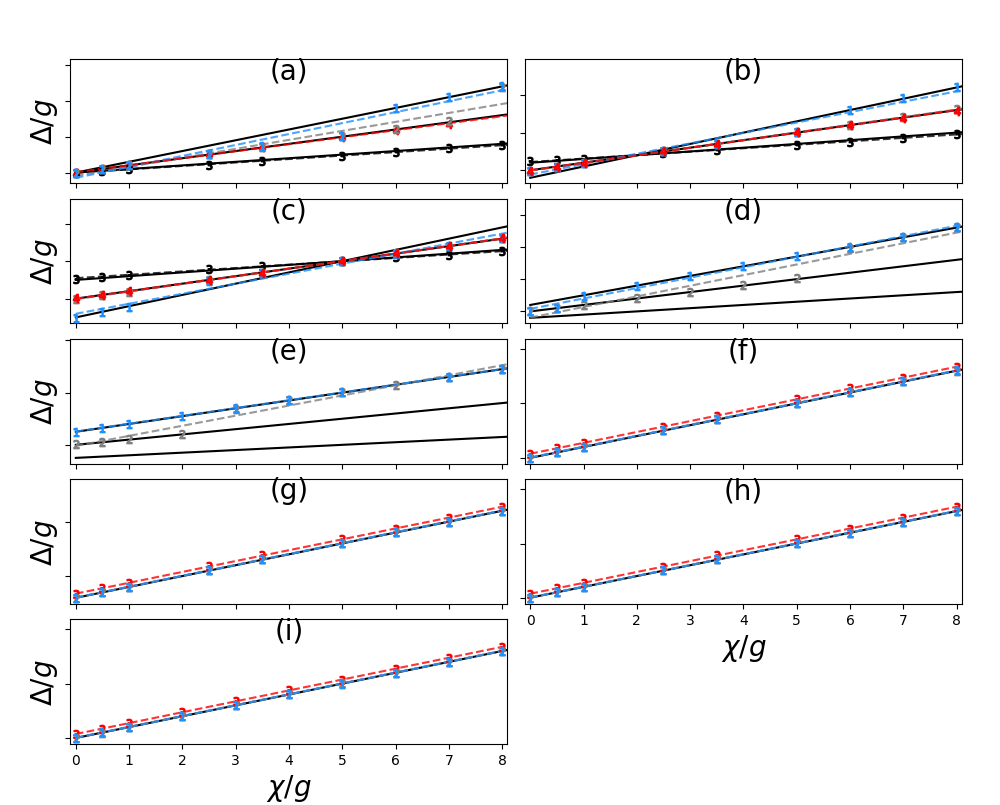
\includegraphics[width=\linewidth]{figuras/ch5/robustez/raices.png}
    \caption{Condiciones de robustez para diferentes estados iniciales y valores de $k-J$. Los puntos representan las raíces de $\delta\phi_g=\phi_d-\phi_u$. Los paneles (a)-(e) son estados iniciales con 2 excitaciones, donde los colores representan el estado inicial: $\ket{gg2}$ en celeste, $\frac{1}{\sqrt{2}}(\ket{eg1}+\ket{ge1})$ en gris, $\ket{ee0}$ en negro y $\frac{1}{\sqrt{2}}(\ket{ee0}+{gg2})$ en rojo. En estas, los valores de $k-J$ son: (a) $k-J=0$, (b) $k-J=1g$, (c) $k-J=2.5g$, (d) $k-J=-1g$, (e) $k-J=-2.5g$. Las tres líneas negras son las condiciones de robustez predichas, donde la de mayor pendiente representa la condición Ec. (\ref{ec4:condicion 1}), la del medio Ec. (\ref{ec4:condicion 2}) y la de menor pendiente, la Ec. (\ref{ec4:condicion 3}). Los paneles (f)-(i) son para las condiciones iniciales de 1 excitación, donde está el $\ket{gg1}$ en celeste, $\frac{1}{\sqrt{2}}(\ket{eg0}+{ge0})$ en gris, y $\frac{1}{\sqrt{2}}(\frac{1}{\sqrt{2}}(\ket{eg0}+{ge0})+gg1)$ en rojo. La línea negra sólida representa la condición de robustez dada por Ec. \ref{ec4:condicion0}. Los valores de $k-J$ son: (f) $k-J=0$, (g) $k-J=1g$, (h) $k-J=2.5g$, (i) $k-J=-2.5g$.}
    \label{fig5:raices}
\end{figure}

El estado inicial $\ket{ee0}$ siempre sigue la condición Ec. (\ref{ec4:condicion 2}), y en presencia del entorno el ajuste predice una modificación aproximada según
\begin{equation}
    \Delta\simeq0.9\chi+2.2(k-J).
    \label{ec5:condicion 2 modificada}
\end{equation}
Los estados iniciales $\ket{gg2}$ y $\frac{1}{\sqrt{2}}(\ket{eg1}+\ket{ge1})$ siguen la condición (\ref{ec4:condicion 3}), y el ajuste en estos casos predice una condición modificada

\begin{equation}
    \Delta\simeq2.05\chi-0.05(k-J).
    \label{ec5:condicion 3 modificada}
\end{equation}
Similarmente, el estado inicial $\frac{1}{\sqrt{2}}(\ket{ee0}+\ket{gg2})$ también sigue la condición 2. Esto nos dice que los estados superposición de la base también siguen estas condiciones. Es interesante que, si bien el estado $\ket{gg2}$ a veces sigue la condición 1, y el $\ket{ee0}$ la 3, su superposición sigue la 2. Este estado es un estado entrelazado, solo si se mira el total del sistema. Si solamente se consideran los dos átomos, esto no es cierto, ya que la cavidad tiene diferente cantidad de excitaciones en cada estado, y por lo tanto al tomar traza parcial las coherencias desaparecen. 

Para los casos de 1 excitación, mostrados en las figuras \ref{fig5:raices}(f)-(i), se ve cómo las dos condiciones iniciales $\frac{1}{\sqrt{2}}(\ket{eg0}+\ket{ge0})$ y $\ket{gg1}$ siguen la única condición de robustez para este subespacio Ec. (\ref{ec3:condicion robuestez 1 atomo}). Sorprendentemente, cuando se considera el estado inicial entrelazado entre ambos estados de la base, $\frac{1}{\sqrt{2}}(\frac{1}{\sqrt{2}}(\ket{eg0}+\ket{ge0})+\ket{gg1})$, entonces presenta un pequeño \textit{offset} con respecto a los otros dos estados de la base. 
\begin{figure}[h]
    \centering
    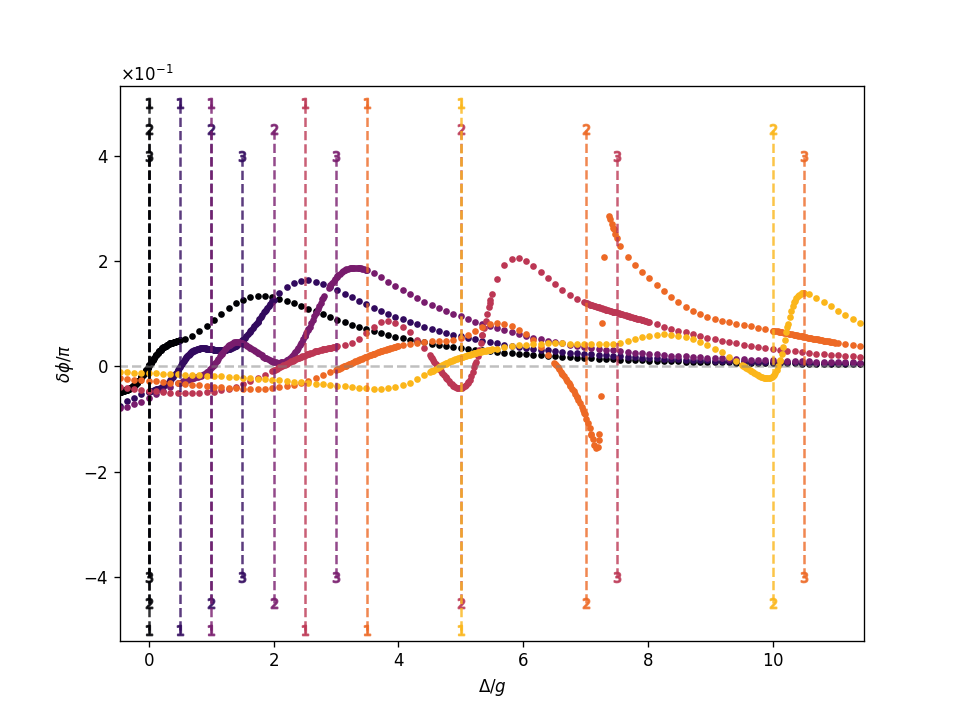
\includegraphics[ width=0.7\textwidth ]{figuras/ch5/robustez/delta-chi/ee0 k=0.0g J=0.0g delta-chi.png} 
    \caption{Diferencia entre la FG unitaria y disipativa para $k-J=0$ y múltiples valores de $\chi\in [0,5g]$. Las líneas rayadas verticales representan las tres posibles condiciones de robustez.}
    \label{fig5:inutil}
\end{figure}



\section{Conclusiones del capítulo 5}

En esta sección se trabajó con la FG en presencia del entorno. Se estudió el efecto de los parámetros del problema y se estudiaron los casos de robustez para distintos estados iniciales. En conclusión se puede decir que las condiciones encontradas predicen los casos de robustez con precisión y sirven en general para cualquier combinación de parámetros, siempre y cuando el estado inicial sea alguno de los estados de la base. 

Por otro lado, se encontraron indicios de que la FG y la concurrencia están relacionadas, ya que ambas siguen las condiciones de robustez. Este mecanismo debe ser algo fundamental y un análisis numérico no es suficiente para determinar cuál es el mecanismo escondido que los relaciona y produce una conservación excepcional de las cantidades estudiadas ante los efectos del entorno. A partir de las simulaciones numéricas utilizadas, se puede concluir que el entorno modifica la condición de robustez. Cuantificar el efecto del entorno requiere un análisis similar al realizado, variando los valores de acoplamiento que excede los objetivos y tiempos de esta Tesis.




